%
% 6.857 homework template
%
% NOTE:
% Be sure to define your team members with the \team command
% Be sure to define the problem set with the \ps command
% Be sure to use the \answer command for each of your answers 
% 
%


\documentclass{article}

\usepackage{amsmath}

\newcommand{\student}{ Xilun Wu }
\newcommand{\PurdueID}{ Wu636 }
\newcommand{\homeworknumber}{ 2 }

%\pagestyle{headings}
%\usepackage[dvips]{graphics,color}
\usepackage{graphicx}
\usepackage{latexsym}
\setlength{\parskip}{1pc}
\setlength{\parindent}{0pt}
\setlength{\topmargin}{-3pc}
\setlength{\textheight}{9.5in}
\setlength{\oddsidemargin}{0pc}
\setlength{\evensidemargin}{0pc}
\setlength{\textwidth}{6.5in}
\newcommand{\problemno}{0}

\newcommand{\newpart}[1]{
\newline
\noindent
(#1)
}

\newcommand{\question}[2]{
\renewcommand{\problemno}{#1}
\newpage
\noindent
\framebox{ \vbox{CS57300 Homework \hfill --- Homework \homeworknumber, Problem #1 --- \hfill  (\today)
  \\ \student (\PurdueID) }}
\bigskip
\newline
\noindent
{\bf Q\problemno :} #2
}

\newcommand{\answer}{
\noindent
\newline
{\bf A:}
\newline
}

\begin{document}

\question{1}{}
\answer 
(i)\quad I agree with Ronald, because we don't have much information about how they sampled the data. The sample method would affect a lot. For example, if the variance of donation amount is large, the randomness of sampling would lead to much difference. Therefore, this doesn't prove anything if the sample space is not large enough or the sampling is not so random. \par
\quad \quad Besides, this is only one-year data, which may not represent the whole situation.
\\\\
(ii)\quad Firstly, I do resample and generate the average of each bin. The distribution is approximate normally, so I choose the run t-test on this data with resampling. \par
\quad \quad Using the data to run one-sided t-test with bin size 200 gives the p-value 0.00012 from which we can reject the null hypothesis that DEM $>$ GOP on average donations. Based on the t-test result, DEM's claim is very likely to be right for year 2012 but unsure for the whole record. 
\\\\
(iii)\quad With the null hypothesis DEM $>$ GOP on average donations, I run t-test on this data by state, and here's the result: {AL, IA, IN, MA, ME, MT, NC, NM, OH, OR, TX} support DEM's claim that DEM $>$ GOP on average donations in state. Other states don't support this claim.

(iv)\quad The sampel size of each state varies a lot which makes them unequal from the perspective of statistics. However, in my solution, we treat each state equally, regradless of weight. This could lead to weakness of the conclusion. \par
\quad \quad In addition, some states get very small sample size, which is inappropriate to be used in t-test. 

(v)\quad {CO, FL, GA, IL, MD, MN, NJ, SC, WA, WV} supports GOP's claim. 
\par
(vi) \par
\quad \quad (Q1.i) The same conclusion as Q1.i. \par
\quad \quad (Q1.ii)  Using the data to run one-sided t-test gives the p-value 0.031 from which we can reject the null hypothesis that DEM $>$ GOP on average donations. Based on the t-test result, DEM's claim is very likely to be right. 
\par
\quad \quad (Q1.iii)  {ID, IL, KS, OH, TX} supports DEM's claim. \par

\question{2}{}
\answer
(i) By CLT, we can do t-test with resampling on data. The result of t-test is:\par
H0: Mean of population1b $>$ Mean of population2b\par
H1: Mean of population1b $<$ Mean of population2b \par

\begin{center}
\begin{tabular}{ |c|c|c| } 
 \hline
 Mean of population1b & Mean of population2b & p-value \\ 
 0.4008919 & 0.4555991 & 6.507e-12 \\ 
 \hline
\end{tabular}
\end{center}
\quad Conclusion: Mean of population1b $<$ Mean of population2b
\par
(ii) By CLT, we can do t-test with resampling on data. The result of t-test is:\par
H0: Mean of population3b $>$ Mean of population4b\par
H1: Mean of population3b $<$ Mean of population4b \par

\begin{center}
\begin{tabular}{ |c|c|c| } 
 \hline
 Mean of population3b & Mean of population4b & p-value \\ 
 0.3596377 & 0.4480959 & 3.618e-05 \\ 
 \hline
\end{tabular}
\end{center}
\quad Conclusion: Mean of population3b $<$ Mean of population4b
\par
(iii) By CLT, we can do t-test directly on data. The result of t-test is:\par
H0: Mean of population1p $=$ Mean of population2p\par
H1: Mean of population1p $\neq$ Mean of population2p \par

\begin{center}
\begin{tabular}{ |c|c|c| } 
 \hline
 Mean of population1p & Mean of population2p & p-value \\ 
 2.666863 & 2.242707 & 0.00657 \\ 
 \hline
\end{tabular}
\end{center}
\quad Conclusion: Mean of population1p $\neq$ Mean of population2p
\par
(iv) By CLT, we can do t-test directly on data. The result of t-test is:\par
H0: Mean of population3p $=$ Mean of population4p\par
H1: Mean of population3p $\neq$ Mean of population4p \par

\begin{center}
\begin{tabular}{ |c|c|c| } 
 \hline
 Mean of population3p & Mean of population4p & p-value \\ 
 2.042834 & 2.542555 & 0.1618 \\ 
 \hline
\end{tabular}
\end{center}
\quad Conclusion: Mean of population3p $=$ Mean of population4p
\par


\question{3}{}
\answer
(i) 
\par
\quad (a) The total rewards are 440. \par
\quad (b) The plot of ucb test is as below: \par
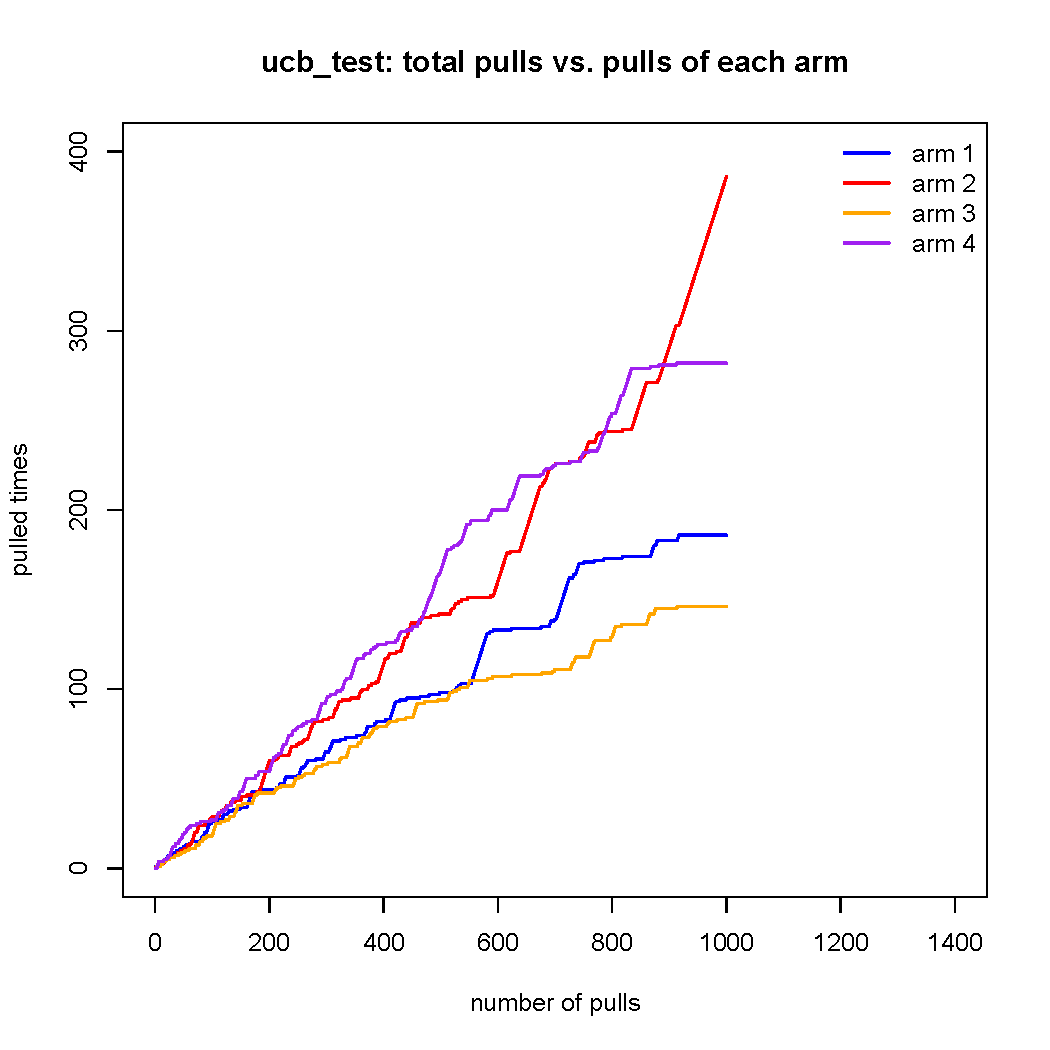
\includegraphics[width=1.0\textwidth]{Q3_1.pdf} 
\\\\
(ii) 
\par
\quad (a) The total rewards are 2629.8. \par
\quad (b) The plot of ucb test is as below: \par
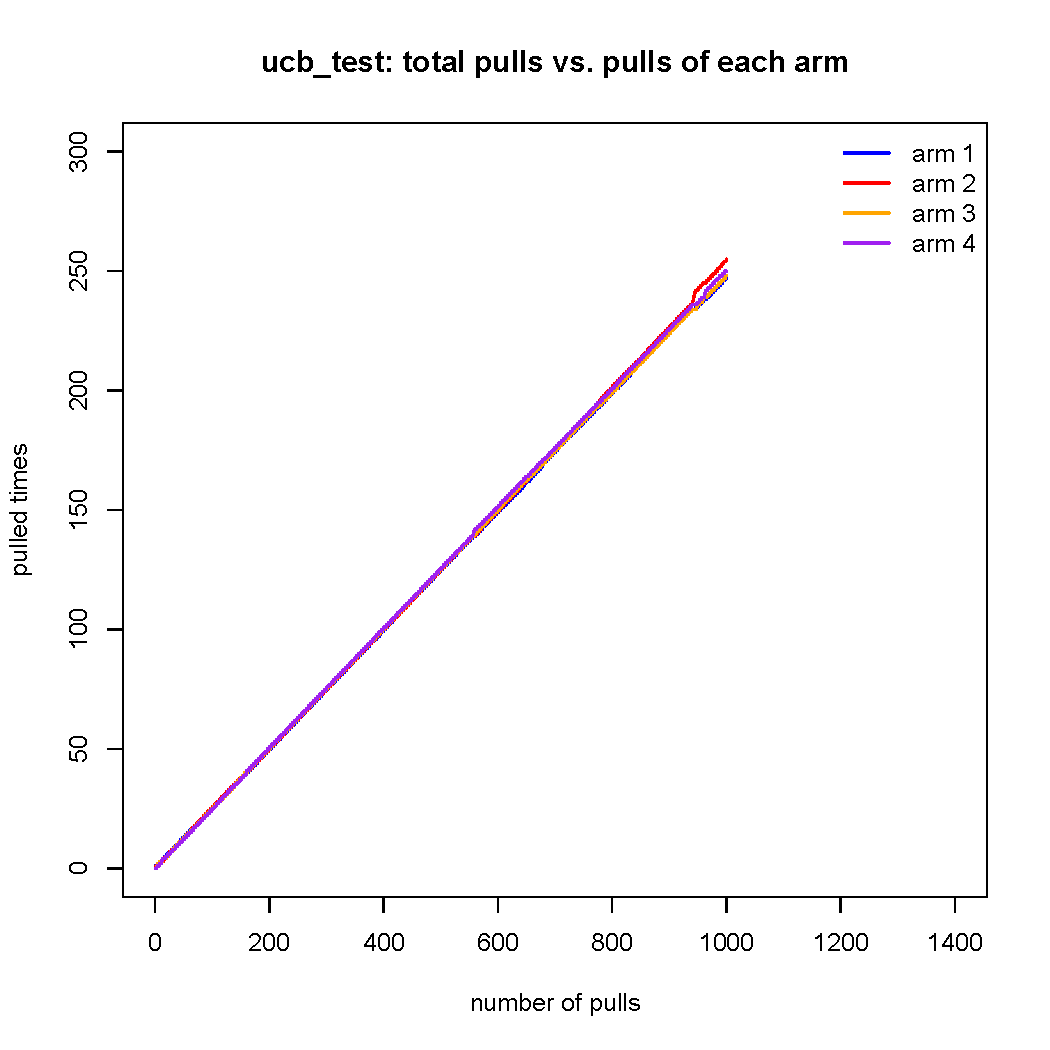
\includegraphics[width=1.0\textwidth]{Q3_2.pdf} 
\\\\
(iii) 
\par
\quad (Redo Q3.i) The total rewards are 420. The plot of epsilon greedy is as below: \par
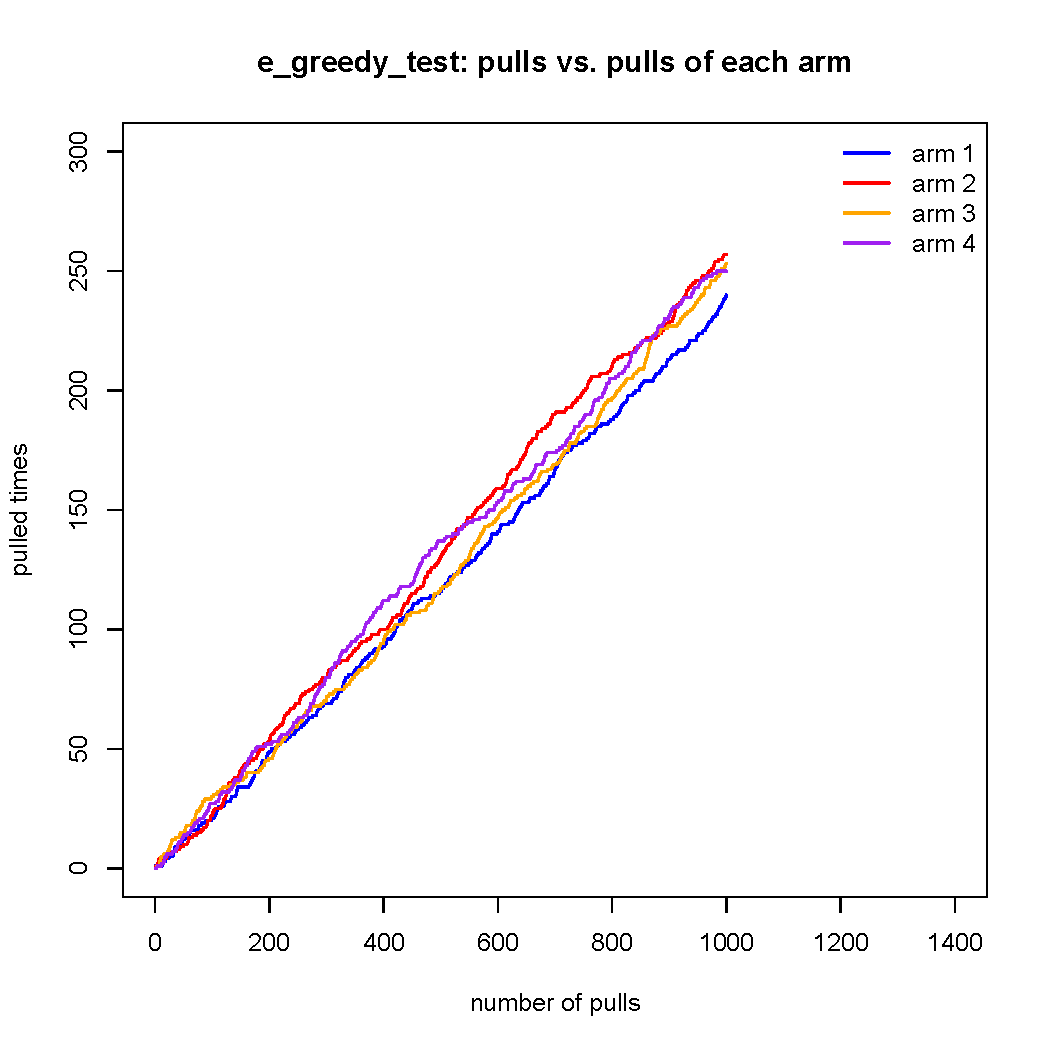
\includegraphics[width=1.0\textwidth]{Q3_3_1.pdf} 
\par
\quad (Redo Q3.ii) The total rewards are 2790.59. The plot of epsilon greedy is as below: \par
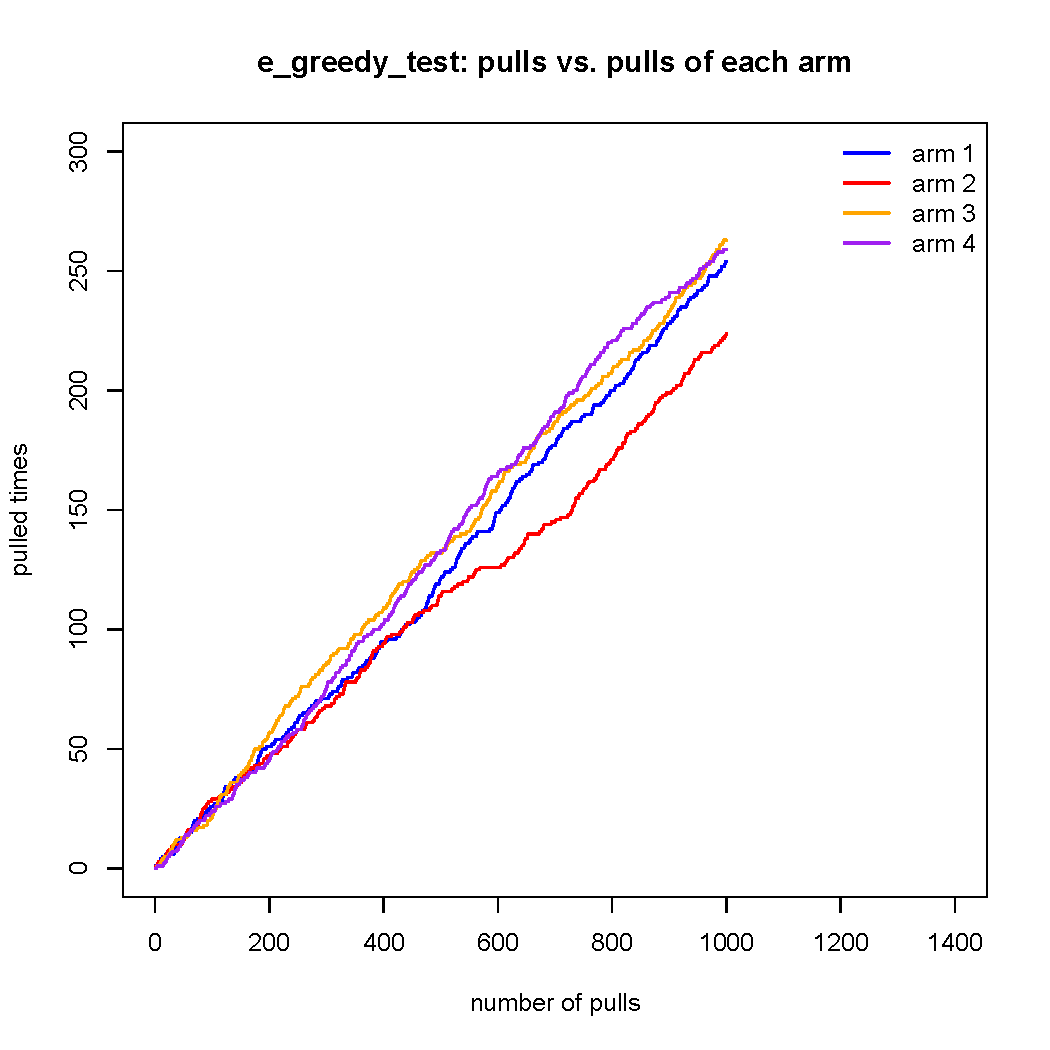
\includegraphics[width=1.0\textwidth]{Q3_3_2.pdf} 
\par
UCB is better for Bernoulli data(populationib.csv) but has poorer performance for real-world data(populationip.csv). 
\par
(iv)
\quad In Q2, we know that population1b $<$ population2b; population3b $<$ population4b; population1p $>$ population2p; population3p and population4p are close(maybe equal). For bernoulli data(populationib), the result of ucb test show the same average relationship as t-test: arm2 has higher expectation than arm1, arm4 has higher expectation than arm3. But for i.i.d unknown random data(populationip), the result of ucb test show that these 4 arms have similar average -- they have very close pulls. I think this is becasue UCB works well for Bernoulli data but has poor performance on real-world problems(data). 
\\\\
(v)
\par
\quad (a) The total rewards are 450. The plot of Thompson Sampling is as below: \par
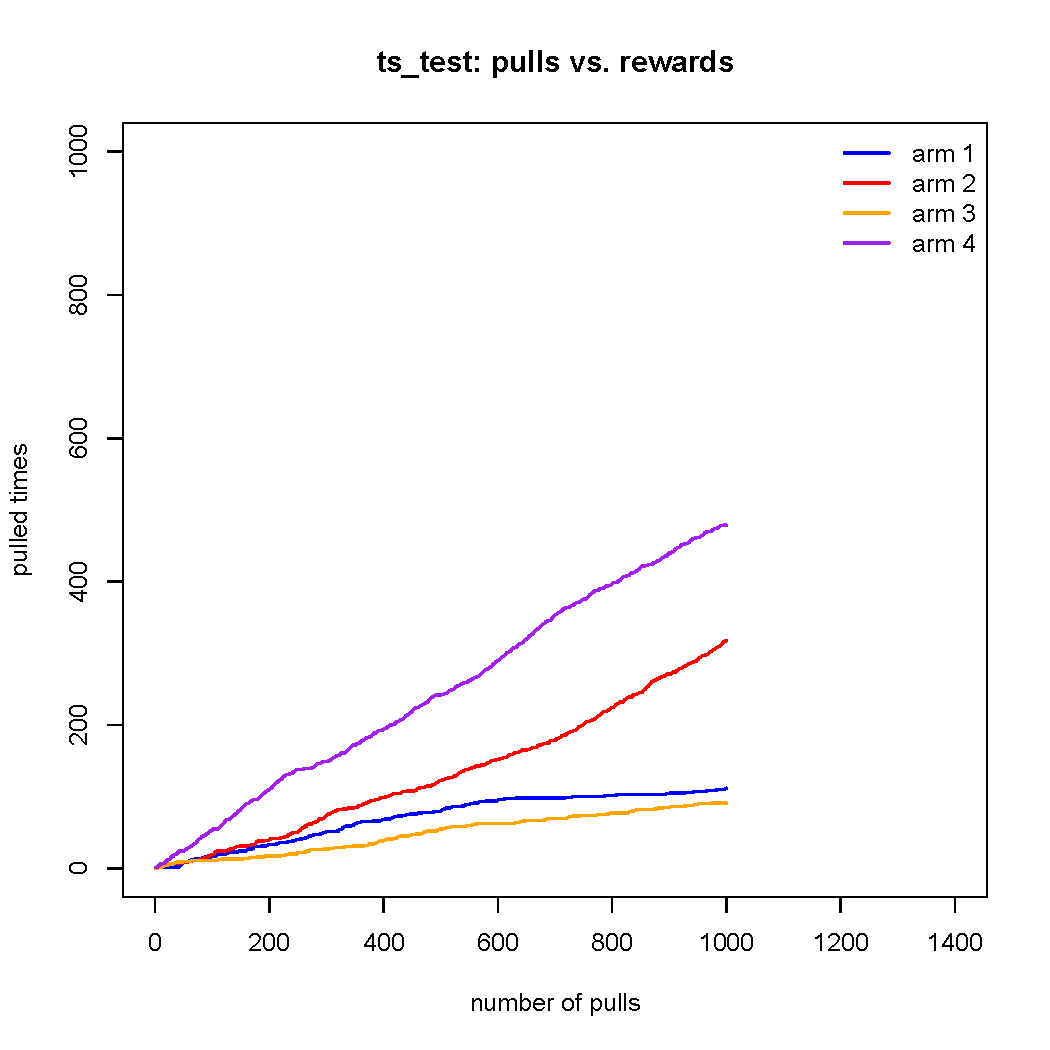
\includegraphics[width=1.0\textwidth]{ts11.pdf} 
\par
\quad (b) The total rewards are 441. The plot of Thompson Sampling is as below: \par
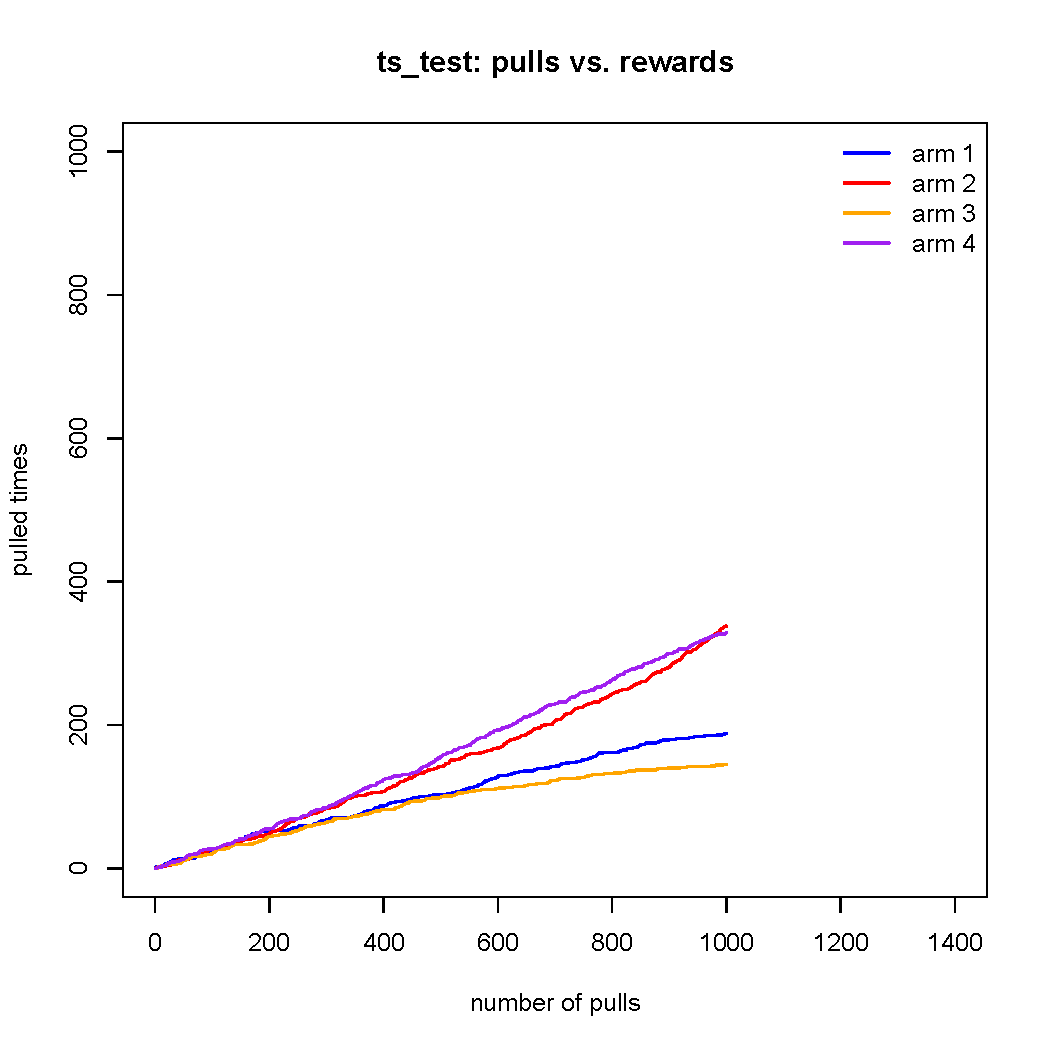
\includegraphics[width=1.0\textwidth]{ts100.pdf} 
\par
\quad (c) \par
\quad Higher the $\alpha, \beta$, tighter is the concentration of Beta($\alpha, \beta$) around the mean.
 As we know, posterior gets concentrated as more samples are obtained, thus higher the $\alpha, \beta$, the later Thompson Sampling could get concentrated(stop being "random"). \par
\quad So, if we want our TS to concentrate later, we can choose large $\alpha, \beta$ like 100, 100, which means we would like our algorithm to get rid of suboptimal at the beginning of test. 
\par
\quad (d) Play-the-winner strategy. 

\end{document}

